\documentclass[a4paper,11pt]{article}
\usepackage{ifpdf} 
\ifpdf
\pdfoutput=1 % if your are submitting a pdflatex (i.e. if you have
             % images in pdf, png or jpg format)
\fi

\usepackage{jcappub}
\usepackage{graphicx}
\graphicspath{{Paper/}{./}}
\usepackage{dcolumn}
\usepackage{amssymb,amsmath,bm}
\usepackage{color}
\usepackage[dvipsnames]{xcolor}
%\usepackage[colorlinks,linkcolor=red,citecolor=blue,urlcolor=blue ]{hyperref}
%\usepackage[utf8]{inputenc}
\usepackage{xfrac}
\usepackage{aas_macros}
\usepackage{mathrsfs}
\usepackage{subcaption}
\usepackage{rotating}
\usepackage{chngcntr}
\newcommand{\nv}{\vec{\theta}}
%\newcommand{\pasj}{Publications of the ASJ}
%\newcommand{\aap}{Astronomy and Astrophysics}
%\newcommand{\apj}{Astrophysical Journal}
%\newcommand{\apjs}{Astrophysical Journal, Supplement}
%\newcommand{\mnras}{Monthly Notices of the RAS}
\newcommand{\todo}[1]{{\bf TODO: #1}}

\newcommand{\as}[1]{{\textcolor{blue}{[AS: #1]}}}
\newcommand{\an}[1]{{\textcolor{magenta}{[AN: #1]}}}
\newcommand{\da}[1]{{\textcolor{red}{[DA: #1]}}}

\newcommand{\vd}{\mathbf{d}}
\newcommand{\vt}{\mathbf{t}}
\newcommand{\vN}{\mathbf{N}}

\newcommand\Tstrut{\rule{0pt}{3ex}}   

%\usepackage{lineno}
%\linenumbers

\definecolor{internationalkleinblue}{rgb}{0.0, 0.18, 0.65}
\hypersetup{urlcolor=internationalkleinblue, linkcolor=internationalkleinblue, citecolor=internationalkleinblue}

\usepackage[T1]{fontenc} % if needed
\usepackage{natbib}
\bibliographystyle{JHEP}
\title{Marginalization of photometric redshift uncertainties}

\author[a,1]{Boryana Hadzhiyska,}
\author[b]{David Alonso,}
\author[c]{Andrina Nicola,}
\author[d]{An\v{z}e Slosar,}

\affiliation[a]{Harvard-Smithsonian Center for Astrophysics, 60 Garden St., Cambridge, MA 02138, USA}
\affiliation[b]{Department of Physics, University of Oxford, Denys Wilkinson Building, Keble Road, Oxford OX1 3RH, United Kingdom}
\affiliation[c]{Department of Astrophysical Sciences, Princeton University, Peyton Hall, Princeton NJ 08544-0010, USA}
\affiliation[d]{Brookhaven National Laboratory, Physics Department, Upton, NY 11973, USA}
\emailAdd{boryana.hadzhiyska@cfa.harvard.edu}

\abstract{We present a new method for marginalization over uncertainties in redshift distributions of tomographic bins applicable to current and coming photometric galaxy surveys. We allow for arbitrary deviations from the best guess $N(z)$ governed by a general covariance matrix describing incompleteness in our knowledge of redshift distributions. In principle, this is marginalization over potentially hundreds of new parameters describing potential deviations as a function of redshift and tomographic bin. However, by Taylor expanding theory predictions around a fiducial model, we can perform the marginalization analytically, resulting in a modified data covariance matrix. We demonstrate  this method by applying to the galaxy clustering measurements from the Year One of Hyper SupremeCam data demonstrate how we can marginalize over sample-variance of the PZ calibration sample and a large general systematic uncertainty in photometric determination methods. We find that this method gives results that are comparable to the ad-hoc shift and width parameterizations and show that the only deviations that matter are smooth deviations. 
}


\begin{document}
\maketitle
\flushbottom

\section{Introduction}\label{sec:intro}

Photometric galaxy surveys  have the potential of  being transformative in our understanding of the Universe by measuring millions and soon billions of galaxies on the sky. These catalogs can be used to constrain cosmological parameters through measurements of clustering and weak lensing as demonstrated by numerous surveys that have completed observations including  Sloan Digital Sky Survey \cite{astro-ph/0006396}, PanSTARRS \cite{2010SPIE.7733E..0EK}, Kilo-degree Survey \cite{1206.1254}, Dark Energy Survey \cite{1601.00329}, Hyper Suprime-Cam survey \cite{2012SPIE.8446E..0ZM}, and will play a crucial role in the upcoming Vera Rubin Observatory LSST Survey \cite{0912.0201}.

it has been long recognized that the accuracy of photometric surveys relies on the accuracy of photometric redshift distributions and that these are likely to continue to be a dominant source of systematic uncertainty. The crucial quantity is the redshift distribution $N(z)$, which is simply the mean number density of galaxies as a function of redshift for each tomographic sample. It is known that the shape of $N(z)$ delivered by the current photometric redshift codes and subsequent calibrations is insufficient for retiring this source of systematic error completely \cite{1809.01669}. Improving photometric redshift techniques and calibrations is an area of active research \cite{2004.09542}\as{add citations}, but for the foreseable future we will need to rely on marginalization to control residual systematic errors.

The traditional approach is to add nuissiance parameters that shift the best guess $N(z)$ or additionally change its width or a relative contribution from a secondary peak in $N(z)$. This usually works well, but in additional to adding potentially large number of nuissance parameters suffers from model completeness problem: how do we know that any given parameterization encompasses all possible ways in which our best-guess $N(z)$ can be wrong?

In this paper we propose a new technique that performs a marginalization around all possible functional deviations from the best fit $N(z)$. The space of possible deviations in $N(z)$ is described as a Gaussian function and under some controlled approximations, the integrals can be performed analytically. This results in a simple change to the data covariance matrix with a simple explanation: directions in the space of predictions that are degenerate with changes in $N(z)$ are given large variance, which means that information in these direction is not used for inferring the parameters of interest. This then marginalizes over $N(z)$ uncertainty in a robust manner that does not add new niussance parameters.

We applyt this method to the HSC data as an example and  discuss some of the advantages, limitations and possible extensions of this model. 




\section{Theory}

In typical cosmological analysis problem, we are performing a Bayesian inference on the posterior $p({\rm theory} | {\rm data} ) \propto p({\rm data}|{\rm} theory) p({\rm theory})$ with the data likelihood given by 
\begin{equation}
p({\rm data}|{\rm theory}) =  \mathcal{L} \propto  \exp\left [-\frac{1}{2} \chi^2 \right], \label{eq:like}
\end{equation}
where
\begin{equation}
  \chi^2  = (\vd-\vt)^T C^{-1} (\vd-\vt),
\end{equation}
where $\vd$ is the data vectory, typically containing all the summary statistic of interest like correlation functions ot power spectra and $\vt$ the theory vector through which parameter dependence enters. In this set-up the covariance matrix $C$ is fixed (and hence the Gaussian normalization term does not enter equation \ref{eq:like}), which is usually a very good approximation in typical problems that we wish to consider \cite{1811.11584}, but note that the method is easily generalizable to the cases where this is not true.

We can make significant progress without specifying explicitly how theory is calculate given the parameters. It suffices to say that given a set of cosmological parameters, which specify the evolution of the universe and thus matter power spectra as a function of scale and redshift, a set of survey properties, such as number densities and redshift distribution of galaxies and weak lensing sources, we can integrate these into theory predictions $\vt=\vt(\theta)$.

The traditional approach is to add to add nuissance parameters that describe our lack of knowledge of galaxy redshift distribution. A typical approach is to use shift and width parameters  \cite{1706.09359,1912.08209} \as{did DES Y1 have shift/width?},
where redshift distributions $N_i(z)$ are shifted according to
    \begin{equation}
      N_{i}(z) \propto \bar{N}_{i}\left(z_{c,i} + (1 + z_{w, i})(z-z_{c, i}) + \Delta z_{i}\right),
      \label{eq:photo-z-model}
    \end{equation} 
where the index $i$ runs over the number of tomographic samples. Here $N_{i}(z)$ is the true redshift distribution with  $\bar{N}_{i}(z)$ out best estimate of it. The parameters $\Delta z_{i}$ and $z_{w,i}$ account for shifts in the means of the distributions, while $z_{c,i} = \left<z\right>_{\bar{N}_i}$ is the mean redshift to act as a sensible pivot for width changes. The shift and width parameters for each tomographic bin are then inferred and marginalized over together with all other parameters.
    
This approach explicitly marginalizes over the two effects that we think are the two most important systematics stemming from redshift distribution uncertainty. However, it suffers from two problems. First, it is fundamentally ad-hoc. This particular parametric form does not stem from consideration of phometric redshift estimators. There is also no reason to believe why it would be complete in the sense that it captures all relevant effects. The second problem is that it is computationally expensive. For example, in the analysis 
    of \cite{1912.08209}, redshift uncertainty parameters accounted for 8 (2 per 4 tomographic bins) of 14 total parameters in the inference process, i.e. over the half parameters inferred were dealing with redshift.

\subsection{A new approach}
    
In this paper we advocate a different approach. First, let's consider a binned description of $N_i(z)$ in terms of $N_{ij}$, where $i$ index describes the tomographic bin and $j$ is redshift index, so that $N_{ij} = N_i(z_j)$ at some discrete grid of $z_j$. This entire vector can be packed in a vector $\vN$.

We will describe our uncertainty in $\vN$ as a Gaussian
\begin{equation}
  p(\vN) \propto \exp\left[  (\vN - \bar{\vN})^T P^{-1} (\vN -\bar{\vN}) \right],
\end{equation}
where $\hat{\vN}$ is our best guess of redshift distribution $P$ is a matrix of allowed deviations. We will discuss later how $P$ can be determined, but at this point we note that it is a general positive-definite matrix, i.e not necessarily diagonal). Other possible parameterizations are sub-summed in this approach. For example, a general shift-width is allowed with the probability $p(\vN(\Delta z_i, z_{w,i}))$.

We can now write a likelihood for the data in which we explicitly marginalize out all the degrees of freedom associated with $\vN$:
\begin{equation}
\mathcal{L} \propto  \int \exp\left [-\frac{1}{2} (\vd-\vt)^T C^{-1} (\vd-\vt) -\frac{1}{2} (\vN - \bar{\vN})^T P^{-1} (\vN -\bar{\vN}) \right]  d^N\vN, \label{eq:like2}
  \end{equation}
  Note that in the equation above, $\vt=\vt(\theta,\vN)$, where $\theta$ are the remaining parameters. It is this dependence that prevents us from performing what looks like a trivial integral.

  In principle, we could solve this problem by making every single element of vector $\vN$ a part of MCMC chain and simply run the MCMC with $\theta$ and additional hundreds of $\vN$ parameters. Instead, we pull an Eastern-European trick and Taylor expand theory around $\hat{\vN}$:
  \begin{equation}
    \vt(\theta,\vN) = \vt(\theta,\bar{\vN}) + T \left(\vN - \bar{\vN} \right), \label{eq:taylor}
  \end{equation}
  where
  \begin{equation}
    T_{mn} = \frac{\partial t_m}{\partial N_n} \bigg|_{\theta,\hat{\vN}}
  \end{equation}
  The matrix $T$ is the non-square matrix giving derivatives of theory with respect to each element of $\vN$. In other words it contains a full information about how all the correlation functions or power spectra respond to changing $N(z)$ distribution for one tomographic bin at one redshift.

  Substituting Eq. \ref{eq:taylor} into Eq. \ref{eq:like} results in an integral that is now quadratic in $\bar{\vN}$ and can be performed analytically. After collecting terms that are quadratic and linear in $\vN$, performing the Gaussian integral and applying the Woodbury matrix identity, we find:
  \begin{equation}
    \mathcal{L} \propto \frac{1}{|T C^{-1} T^T +P^{-1} |^{1/2}} \exp\left [-\frac{1}{2} (\vd-\vt)^T C_M^{-1} (\vd-\vt) \right], \label{eq:main1}
  \end{equation}
  where
  \begin{equation}
    C_M = C + T PT^T \label{eq:main2}
  \end{equation}
  This is a fascinatingly simple equation and the main result of this paper. This calculation should be understood as follows: for each deviation around $\hat{\vN}$, there is a corresponding deviation around $\vt$. These are directions in space of theory predictions that are perfectly degenerate with the changes in shape of $N(z)$.  Equation \ref{eq:main2}  increases the variance for those linear combinations commensurate with how far P allows them to go.

  In principle, at every point in likelihood, one should evaluate Eq. \ref{eq:main1}, which means recalculating $T$. Since this is a very expensive computation, we will further simplify the problem, by assuming $T$ is only weakly deviations from some fiducial cosmology. We will therefore pre-compute $T$ once for the fiducial cosmology, which then means that normalization term in equation \ref{eq:main1} is an irrelevant constant and at fixed data covariance matrix $C$, the Eq. \ref{eq:main2} also needs to be evaluated just once.

  The procedure is thus as follows:
  \begin{itemize}
  \item Run inference problem once with fixed redshift distribution to determine a sensible fiducial model.
    
  \item Calculate $T$ and $C_M$ at this fiducial model
    
  \item Re-run inference with the modified covariance matrix $C_M$, which leads to broadened contours due to marginalization of redshift distributions
    
  \end{itemize}
If needed, one could repeat the inference at a refined fiducial model although in pracice we found this to be unnecessary.

Note that there are two distinct approximation here. The first is that theory can validly be Taylor expanded in $\vN-\bar{\vN}$ and the second is that $T$ is model independent for models of interest. We will examine validity of both of those approximations in Section \ref{sec:hsc}.

\subsection{Determination of prior matrix $P$}

Determination of the prior matrix $P$ is where the the actual and often partially subjective prior on our knowledge of $N(z)$ enters. Note that the standard parameterizations can always be recast in this language at least in the perturbative limits. For example, a vector of derivatives $\lambda_i = dN_i/dz$ when added to $\vN$ will produce a shift in the the shape of $N_i(z)$. Therefore, adding a contribution $\sigma_{zi}^2 \lambda_i \lambda_i^T$ will allow shifts with variance $\sigma_{zi}$. Of course, when shifts become so large that the perturbative expansion breaks, the approach will work only approximately. But in this paper we are not interesting in shifts; instead we will try to build $P$ is a more systematic manner. 


\subsubsection{Uncertainty due to estimator biases}
We will build $P$ from three pieces. The first piece is simply the overall uncertainty stemming from the fact that the photometric redshift estimators have errors. The simplest thing is to make this covariance matrix   \ldots


\subsubsection{Cosmic Variance in calibrator sample}
The covariance matrix between two tomographic bins is given by:
\begin{equation}
Cov_{ij}=\frac{N_i N_j}{2\pi^2} \int_0^\infty dk_\parallel \cos(k_\parallel(\chi_i-\chi_j))\int_0^\infty dk_\perp k_\perp W_i(k_\parallel,k_\perp)W_j(k_\parallel,k_\perp)P_{\bf gg}({\bf k}),
\end{equation}
where we can model the power spectra at each bin centre and for all
transverse and parallel modes using the Kaiser formula (CITE), which corrects for redshift space distortions through
the expression:
\begin{equation}
P_{gg}({\bf k},z)=\left(b_g(z)+f(z)\frac{k_\parallel^2}{k^2}\right)^2\,P_{mm}(k,z),
\end{equation}
where $f(z)$ is
the logarithmic growth
rate
and the
evolution of the linear galaxy bias is given by $b_g(z) = 0.95/D(z)$
with $D(z)$ the growth factor.

In this work, we use the galaxy sample in the COSMOS survey as calibrator, which
covers a total area of
$A_{\rm sky} = 1.7 \ {\rm deg}^2$ for galaxies with redshifts $z < 2$.
We model the window function for each bin of the dataset through:
\begin{equation}
W(k_\parallel,k_\perp)=j_0(k_\parallel\Delta\chi/2)\,\frac{2 J_1(k_\perp R_{\rm mean})}{k_\perp R_{\rm mean}},
\end{equation}
where $R_{mean}$ is the
physical size of the survey measured at the mean
distance to the
tomographic bin, 
$R_{\rm mean} = 
\sqrt{\frac{A_{\rm sky}}{\pi}} \chi_{\rm mean}$.
We assume that the
cosmic covariance
between the tomographic bins is negligible, so we estimate the cosmic variance covariance matrix by
treating each bin independently. We show the resulting correlation matrix of the COSMOS cosmic variance in Fig. \ref{fig:CV}.

\begin{figure}[ht]
\centering  
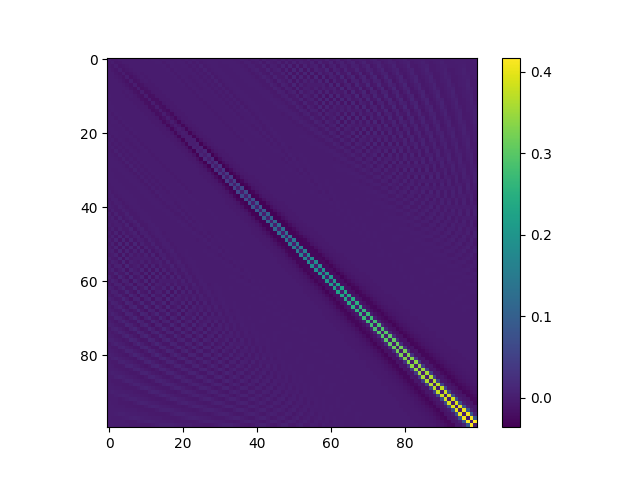
\includegraphics[width=1.\textwidth]{./corr_CV_0.png}
\caption{Cosmic variance (CV) correlation matrix with subtracted diagonal for the first tomographic bin of the HSC data.} 
\label{fig:CV}
\end{figure}


\subsubsection{Smoothness prior}


  





\section{Appplication to HSC clustering data}
\label{sec:hsc}
\an{Some citations are currently missing but I will put them in later.}
We apply the method outlined above to the data obtained in Ref.~\cite{1912.08209}. This work measured the angular galaxy clustering power spectrum from HSC DR1 data. In the following, we give a very brief summary of the methodology employed in this work and refer the reader to Ref.~\cite{1912.08209} for more details.
\subsection{Background theory}
The angular clustering signal for galaxies in redshift bins $i, j$ with photo-$z$ distributions $p^i(z), p^j(z)$ can be modeled using the Limber approximation as \cite{1953ApJ...117..134L, 1992ApJ...388..272K, Kaiser:1998}
    \begin{equation}\label{eq:cell_gg_limber}
      C^{ij}_\ell = \int \mathrm{d}z\,\frac{H(z)}{\chi^2(z)} p^i(z)p^j(z)\,P_{gg}\left(z,k=\frac{\ell+1/2}{\chi(z)}\right),
    \end{equation}
where $P_{gg}(z,k)$ denotes the underlying 3D galaxy power spectrum, $\chi(z)$ is the comoving distance and $H(z)$ denotes the Hubble parameter at redshift $z$. As can be seen from Eq.~\ref{eq:cell_gg_limber}, the spherical harmonic power spectrum $C_{\ell}$ depends linearly on the photometric redshift distributions $p^i(z)$, which facilitates the computation of the $T$ matrix defined above. 

We follow Ref.~\cite{1912.08209} and compute theoretical predictions for the galaxy power spectrum $P_{gg}(z,k)$ within the halo model combined with halo occupation distribution modeling \cite{2000MNRAS.318.1144P,2002PhR...372....1C,2002ApJ...575..587B,2005ApJ...633..791Z,2013MNRAS.430..725V}. 
\subsection{The HSC dataset}
The Hyper-Suprime Cam survey is an on-going photometric galaxy survey survey focused mainly on weak gravitational lensing. The analysis in Ref.~\cite{1912.08209} is based on the publicly-available HSC DR1 data, whose so-called wide fields cover approximately 108 square degrees on the sky, subdivided into seven distinct patches. Ref.~\cite{1912.08209} used these data to compute spherical harmonic galaxy clustering power spectra for four tomographic redshift bins between $z=0.15$ and $z=1.5$, taking both auto- and cross-correlations into account. These power spectra have been corrected for observational and extragalactic systematics by deprojection at the map-level \cite{2019MNRAS.484.4127A}. Finally, following Ref.~\cite{2019PASJ...71...43H}, photometric redshift distributions have been estimated by cross-matching HSC galaxies to galaxies in the COSMOS 30-band photometric catalog presented in Ref.~\cite{2016ApJS..224...24L}.
\subsection{Validating the linear expansion}


\begin{figure}[ht]
\centering  
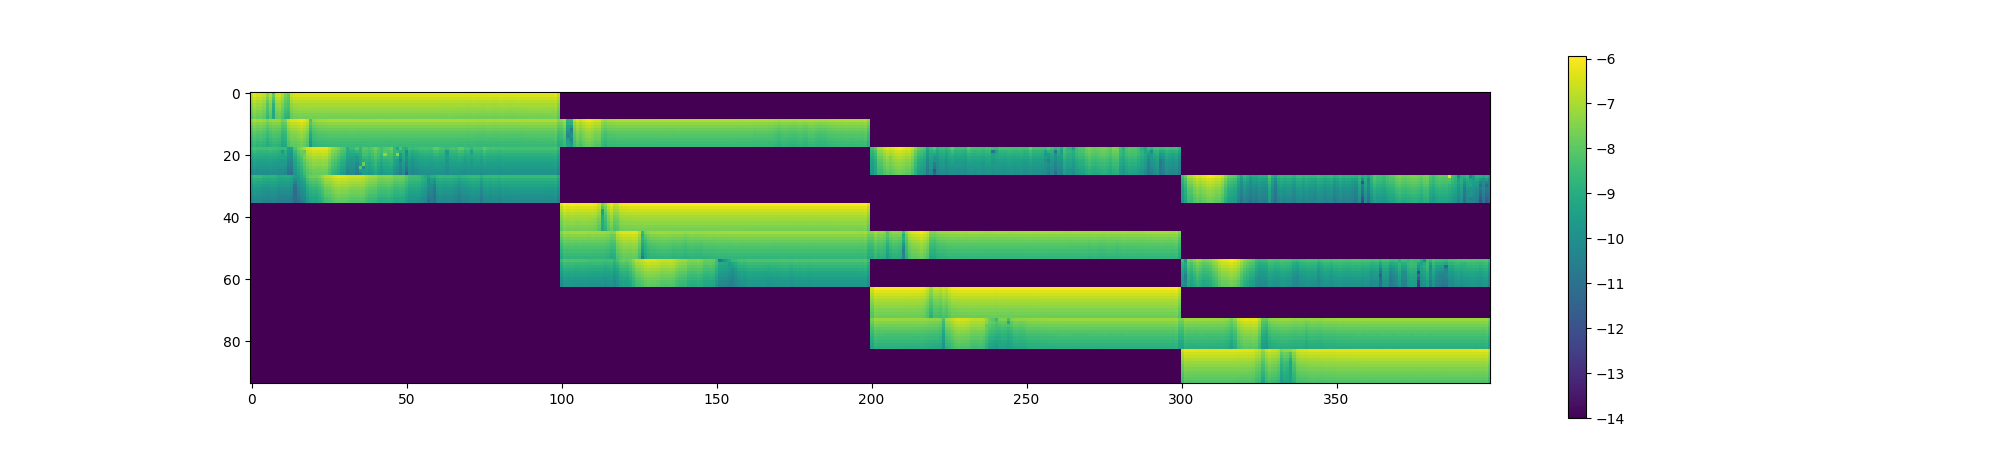
\includegraphics[width=1.2\textwidth]{./Tmat.png}
\caption{Visualization of the derivative matrix $T_{mn} = {\partial t_m}/{\partial N_n}$. \todo{Make look nicer: split into tomo bins}} 
\label{fig:Tmat}
\end{figure}

\begin{itemize}
  \item Plot showing $T$
  \item Plot showing exact $C_\ell$ vs linear prediction. \todo{Make your plots into subplots; verify the Tmatrix}
\end{itemize}{}
\subsection{Impact of N(z) uncertainties on final parameters}


\begin{figure}[ht]
\centering
\begin{subfigure}{.5\textwidth}
  \centering
  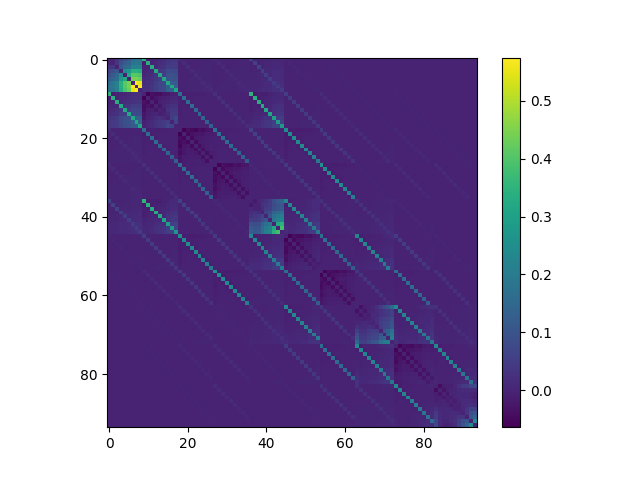
\includegraphics[width=1.\linewidth]{./corr_data.png}
  \label{fig:sub1}
\end{subfigure}%
\begin{subfigure}{.5\textwidth}
  \centering
  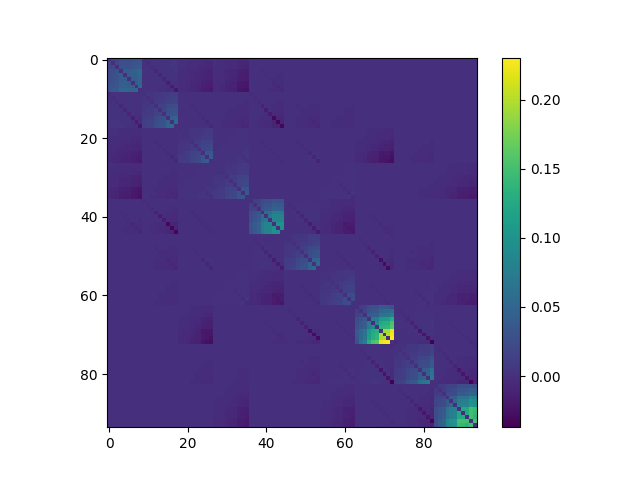
\includegraphics[width=1.\linewidth]{./corr_diff.png}
  \label{fig:sub2}
\end{subfigure}
\caption{Correlation matrix for the fiducial HSC dataset (\textit{left}) and difference with its marginalized version (\textit{right}).}
\label{fig:fid_marg_cov}
\end{figure}

\begin{figure}[ht]
\centering  
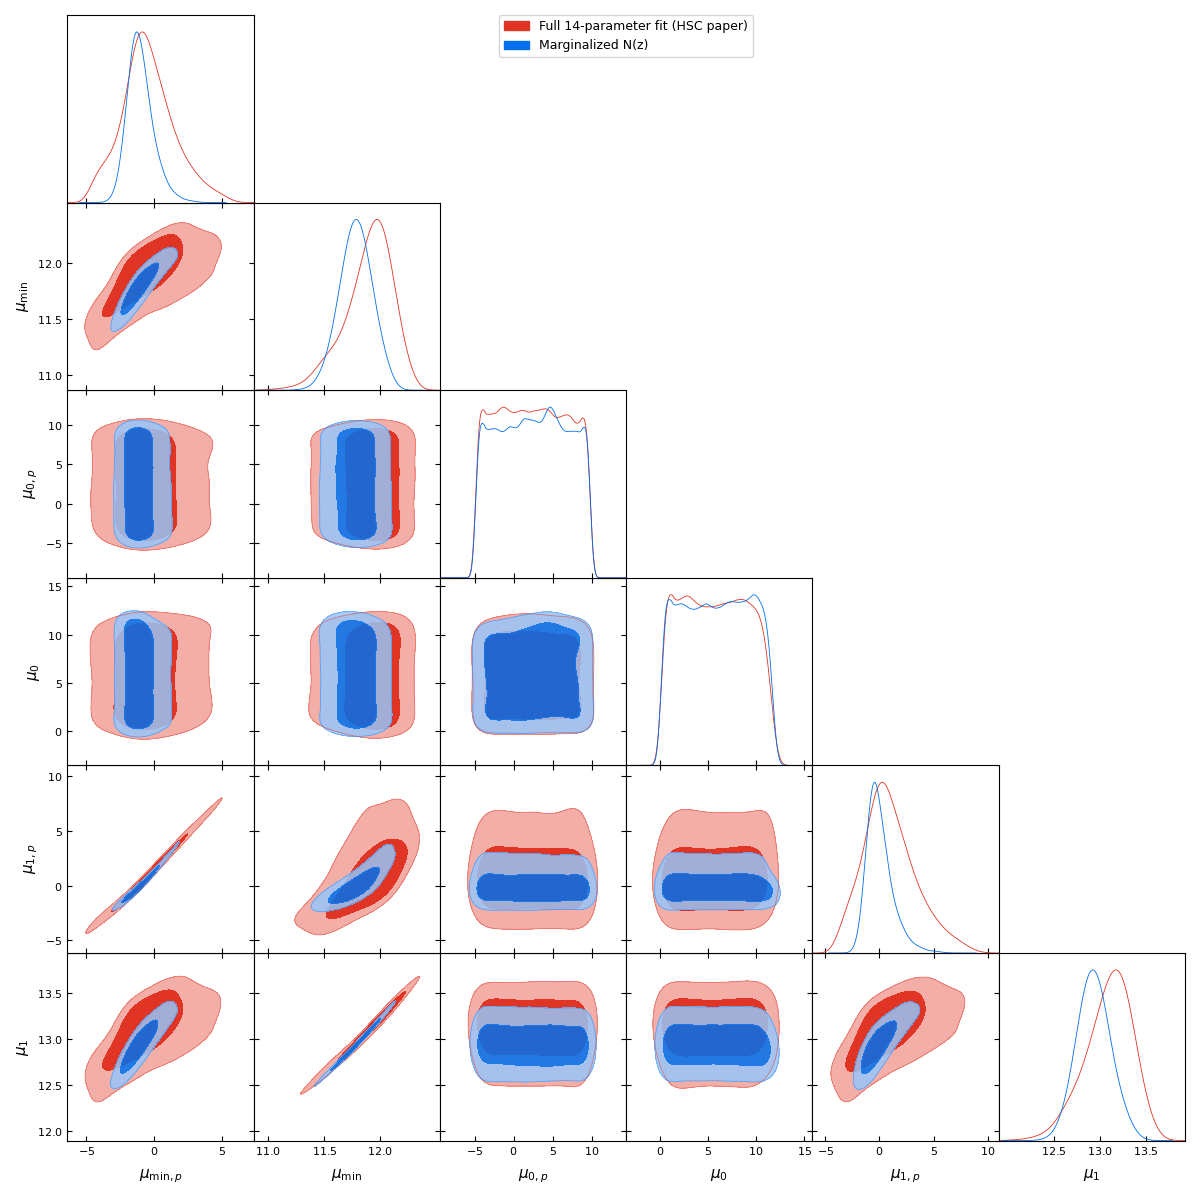
\includegraphics[width=1.\textwidth]{./triangle_fid_marg.png}
\caption{Triangle plot with constraints of the 6 HOD parameters obtained using the covariance matrix from the full HSC dataset (\textit{red}) and from its marginalized version (\textit{blue}).}
\label{fig:triangle_fid_marg}
\end{figure}

\begin{figure}[ht]
\centering  
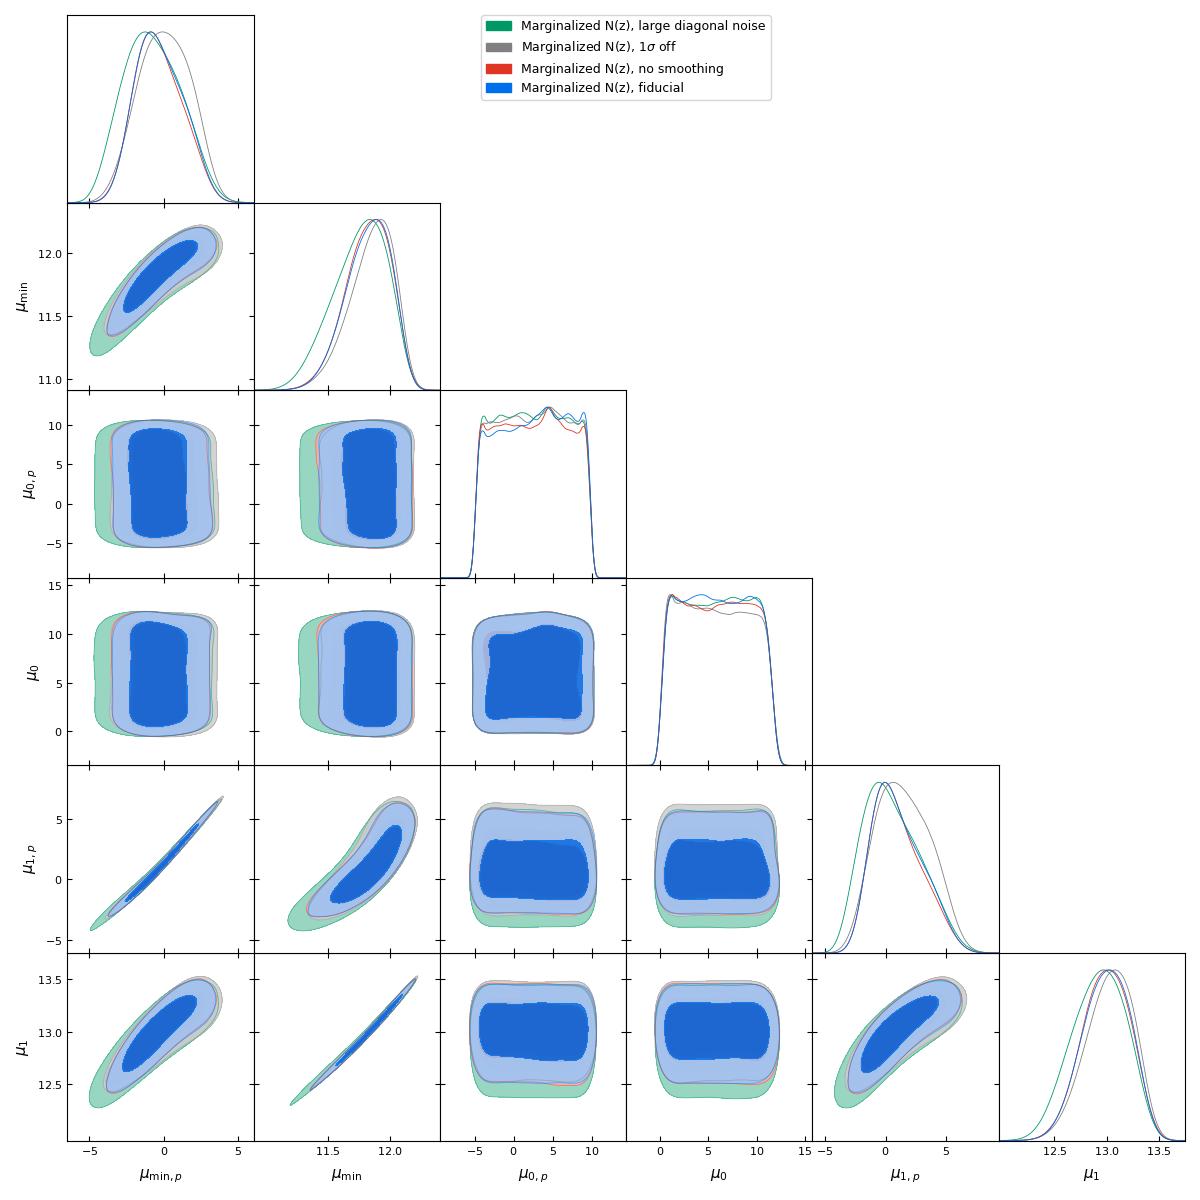
\includegraphics[width=1.\textwidth]{./triangle_marg_tests.png}
\caption{Triangle plot with constraints of the 6 HOD parameters obtained using different choices for the marginalized covariance matrix: in \textit{green} is shown the result where the diagonal noise is set to a very large value ($A_{\rm noise} = 42$); in \textit{gray} is shown the case where the marginalization is performed assuming fiducial HOD-model values which are $1\sigma$ away from their posterior mean values taken from \todo{CITE Andrina's paper}; in \textit{red} is shown the case where the smoothing has been removed ($A_{\rm smooth} = 0$); and finally in \textit{blue} is shown the fiducial case with $A_{\rm noise} = 4$ and $A_{\rm smooth} = 0.25$.}
\label{fig:triangle_marg_tests}
\end{figure}

Plots showing the effects of different things:
\begin{itemize}
\item Compare different choices of prior (smoothness, no smoothing, different degrees of noise etc.)
\item Triangle plot with T matrix computed from a different fiducial.
\item Compare CV-only covariance vs. no covariance.
\item Compare old marginalization vs. new one (maybe same plot).
\item Compare old marginalization with CV priors (importance sample).
\end{itemize}

Other results:
\begin{itemize}
  \item smoothness does nothing
  \item quote $\chi^2$ values \todo{Make a table}
\end{itemize}



\begin{center}
 \begin{tabular}{c | c c c} 
 \hline\hline
 Parameter & HSC covariance, full & HSC covariance, HOD & Marginalized covariance, HOD \\ [0.5ex] 
 \hline
 $\chi^2/\nu$ & 87.49/80 & 94.97/88 & 91.06/88 \\ 

 $\mu_{{\rm min},p}$ & -0.52 & -1.47 & -1.42 \\

 $\mu_{\rm min}$ & 11.88 & 11.73 & 11.73 \\

 $\mu_{0,p}$ & 1.68 & 4.86 & 5.03 \\
 
 $\mu_{0}$ & 0.02 & 11.53 & 11.41 \\

 $\mu_{1,p}$ & 0.87 & -0.58 & -0.51 \\

 $\mu_{1}$ & 13.073 & 12.866 & 12.873 \\ [1ex] 
 \hline
 \hline
\end{tabular}
\end{center}
%[-1.42408101 11.73454764  5.0302023  11.41301207 -0.50980494 12.87323354]
%[-1.47048791 11.73097558  4.85774675 11.52813388 -0.58053445 12.86613972]
%[ 2.18173486e-02 -1.39414027e-02 -4.61928378e-03  1.27879857e-02
% -5.18739083e-01  1.18844059e+01  1.67767553e+00  2.01822301e-02
%  8.65219859e-01  1.30726966e+01 -1.64307267e-01 -3.19342441e-02
%  3.97310971e-02  3.88321407e-02]


\section{Conclusions}


\bibliography{bibliography}

\end{document}
